\chapter{Specifikacija programske potpore}
		
	\section{Funkcionalni zahtjevi}
			
%			\textbf{\textit{dio 1. revizije}}\\
			
%			\textit{Navesti \textbf{dionike} koji imaju \textbf{interes u ovom sustavu} ili  \textbf{su nositelji odgovornosti}. To su prije svega korisnici, ali i administratori sustava, naručitelji, razvojni tim.}\\
				
%			\textit{Navesti \textbf{aktore} koji izravno \textbf{koriste} ili \textbf{komuniciraju sa sustavom}. Oni mogu imati inicijatorsku ulogu, tj. započinju određene procese u sustavu ili samo sudioničku ulogu, tj. obavljaju određeni posao. Za svakog aktora navesti funkcionalne zahtjeve koji se na njega odnose.}\\
			
			
			\noindent \textbf{Dionici:}
			
			\begin{packed_enum}
				
				\item Naručitelj
				\item Administrator
				\item Neregistrirani korisnik	
				\item Registrirani korisnik
				\item Razvojni tim
				
			\end{packed_enum}
			
			\noindent \textbf{Aktori i njihovi funkcionalni zahtjevi:}
			
			
			\begin{packed_enum}
				\item  \underbar{Administrator (inicijator) može:}
				
				\begin{packed_enum}
					
					\item dodati autore, radove, pokrovitelje konferencije i lokacije
					\item uređivati podatke konferencije
					\item započeti i završiti konferenciju
					\item postaviti fotografije koje su slikane tijekom konferencije u galeriju
					\item objaviti rezultate konferencije
					
				\end{packed_enum}
			
				\item  \underbar{Neregistrirani korisnik (inicijator) može:}
				
				\begin{packed_enum}
					
					\item pristupiti sustavu
					\item unijeti lozinku za pristup konferenciji
					\item registrirati se u sustav
					
				\end{packed_enum}
				
				\item  \underbar{Registrirani korisnik (inicijator) može:}
				
				\begin{packed_enum}
					
					\item prijaviti se u sustav
					\item pregledavati promotivne materijale pokrovitelja konferencije
					\item pregledavati radove sudionika
					\item glasati za jedan rad
					\item uz pomoć direktnog video prijenosa pratiti trenutna događanja u glavnoj konferencijskoj dvorani
					\item pregledavati i spremati fotografije iz galeriji
					\item vidjeti mjesto održavanje konferencije i podatke o trenutnim vremenskim uvjetima
					\item vidjeti konačne rezultate konferencije
					
				\end{packed_enum}
					
				\item  \underbar{Baza podataka (sudionik) obavlja:}
					
				\begin{packed_enum}
						
					\item pohranjuje sve podatke o korisnicima
					\item pohranjuje sve podatke o autorima i njihovim radovima
					\item pohranjuje sve podatke o konferencijama
					\item pohranjuje sve podatke o mjestu održavanja
					\item pohranjuje sve podatke o fotografijama slikanim tijekom konferencije i pokroviteljima
						
				\end{packed_enum}
				
			\end{packed_enum}
			
			\eject 
			
			
				
			\subsection{Obrasci uporabe}
				
%				\textbf{\textit{dio 1. revizije}}
				
%				\subsubsection{Opis obrazaca uporabe}
				
%					\noindent \underbar{\textbf{UC$<$broj obrasca$>$ -$<$ime obrasca$>$}}
%					\begin{packed_item}
	
%						\item \textbf{Glavni sudionik: }$<$sudionik$>$
%						\item  \textbf{Cilj:} $<$cilj$>$
%						\item  \textbf{Sudionici:} $<$sudionici$>$
%						\item  \textbf{Preduvjet:} $<$preduvjet$>$
%						\item  \textbf{Opis osnovnog tijeka:}
						
%						\item[] \begin{packed_enum}
	
%							\item $<$opis korak jedan$>$
%							\item $<$opis korak dva$>$
%							\item $<$opis korak tri$>$
%							\item $<$opis korak četiri$>$
%							\item $<$opis korak pet$>$
%						\end{packed_enum}
						
%						\item  \textbf{Opis mogućih odstupanja:}
						
%						\item[] \begin{packed_item}
	
%							\item[2.a] $<$opis mogućeg scenarija odstupanja u koraku 2$>$
%							\item[] \begin{packed_enum}
								
%								\item $<$opis rješenja mogućeg scenarija korak 1$>$
%								\item $<$opis rješenja mogućeg scenarija korak 2$>$
								
%							\end{packed_enum}
%							\item[2.b] $<$opis mogućeg scenarija odstupanja u koraku 2$>$
%							\item[3.a] $<$opis mogućeg scenarija odstupanja  u koraku 3$>$
							
%						\end{packed_item}
%					\end{packed_item}

					\noindent \underbar{\textbf{UC1 - Stvaranje konferencije i dodjela administratora}}
					\begin{packed_item}
	
						\item \textbf{Glavni sudionik: }Super Administrator
						\item  \textbf{Cilj:} Stvoriti konferenciju i dodijeliti je administratoru.
						\item  \textbf{Sudionici:} Baza podataka
						\item  \textbf{Preduvjet:} -
						\item  \textbf{Opis osnovnog tijeka:}
						
						\item[] \begin{packed_enum}
	
							\item Super Administrator stvara konferenciju.
							\item Pridjeljuje ovlasti nad konferencijom odabranom administratoru.
						\end{packed_enum}
						
						\item  \textbf{Opis mogućih odstupanja:}
						
						\item[] \begin{packed_item}
	
							\item[2.a] Administrator ne postoji
							\item[] \begin{packed_enum}
								
								\item Super Administrator stvara Administratora i ponavlja postupak.
								
							\end{packed_enum}
							
						\end{packed_item}
					\end{packed_item}

					\noindent \underbar{\textbf{UC2 - Unos podataka o konferenciji}}
					\begin{packed_item}
						
						\item \textbf{Glavni sudionik: }Administrator
						\item  \textbf{Cilj:} Dodati podatke o konferenciji u bazu podataka.
						\item  \textbf{Sudionici:} Baza podataka
						\item  \textbf{Preduvjet:} -
						\item  \textbf{Opis osnovnog tijeka:}
						
						\item[] \begin{packed_enum}
							
							\item Administrator unosi podatke o konferenciji i mjestu održavanja.
							\item Podaci se pohranjuju u bazu podataka.
					
						\end{packed_enum}
							
					\end{packed_item}

					\noindent \underbar{\textbf{UC3 - Unos podataka o autoru i radu}}
					\begin{packed_item}
						
						\item \textbf{Glavni sudionik: }Administrator
						\item  \textbf{Cilj:} Dodati podatke o autoru i radu u bazu podataka.
						\item  \textbf{Sudionici:} Baza podataka
						\item  \textbf{Preduvjet:} -
						\item  \textbf{Opis osnovnog tijeka:}
						
						\item[] \begin{packed_enum}
							
							\item Administrator unosi podatke o autoru i radu preko grafičkog sučelja.
							\item Aplikacija dodaje podatke u bazu podataka.
					
						\end{packed_enum}
		
					\end{packed_item}

					\noindent \underbar{\textbf{UC4 - Početak konferencije}}
					\begin{packed_item}
						
						\item \textbf{Glavni sudionik: }Administrator
						\item  \textbf{Cilj:} Omogućiti korisnicima pristup konferenciji, pregled radova i glasovanje.
						\item  \textbf{Sudionici:} Baza podataka
						\item  \textbf{Preduvjet:} Uneseni su svi potrebni podaci o konferenciji.
						\item  \textbf{Opis osnovnog tijeka:}
						
						\item[] \begin{packed_enum}
							
							\item Administrator započinje konferenciju.

						\end{packed_enum}
							
					\end{packed_item}

					\noindent \underbar{\textbf{UC5 - Dodavanje fotografija u galeriju}}
					\begin{packed_item}
						
						\item \textbf{Glavni sudionik: }Administrator
						\item  \textbf{Cilj:} Dodati fotografije konferencije u galeriju.
						\item  \textbf{Sudionici:} Baza podataka
						\item  \textbf{Preduvjet:} Konferencija postoji.
						\item  \textbf{Opis osnovnog tijeka:}
						
						\item[] \begin{packed_enum}
							
							\item Administrator tijekom i nakon konferencije dodaje fotografije pomoću grafičkog sučelja.
							\item Aplikacija pohranjuje osnovne podatke o fotografijama u bazu podataka.

						\end{packed_enum}
							
					\end{packed_item}
					
					\noindent \underbar{\textbf{UC6 - Registracija}}
					\begin{packed_item}
						
						\item \textbf{Glavni sudionik: }Neregistrirani korisnik
						\item  \textbf{Cilj:} Registrirati se u sustavu kako bi se omogućio pristup svim funkcionalnostima aplikacije.
						\item  \textbf{Sudionici:} Baza podataka
						\item  \textbf{Preduvjet:} Korisnik ima dobiven pin.
						\item  \textbf{Opis osnovnog tijeka:}
						
						\item[] \begin{packed_enum}
							
							\item Korisnik pristupa registracijskoj stranici aplikacije.
							\item Unosi svoje osobne podatke za registraciju.
							\item Sustav provjerava podatke i stvara račun.
							\item Korisnik prima potvrdu o uspješnoj registraciji i pristupa stranici konferencije.
						\end{packed_enum}
						
						\item  \textbf{Opis mogućih odstupanja:}
						
						\item[] \begin{packed_item}
							
							\item[3.a] Uneseni podaci nepotpuni ili neispravni.
							\item[] \begin{packed_enum}
								
								\item Sustav prikazuje upozorenje i traži ispravak podataka.
								
							\end{packed_enum}
						\end{packed_item}
					\end{packed_item}
					
					\noindent \underbar{\textbf{UC7 - Prijava u sustav}}
					\begin{packed_item}
						
						\item \textbf{Glavni sudionik: }Registrirani korisnik
						\item  \textbf{Cilj:} Prijaviti se u sustav kako bi se pristupilo konferenciji.
						\item  \textbf{Sudionici:} Baza podataka
						\item  \textbf{Preduvjet:} Korisnik ima korisnički račun.
						\item  \textbf{Opis osnovnog tijeka:}
						
						\item[] \begin{packed_enum}
							
							\item Korisnik pristupa stranici za prijavu u aplikaciju.
							\item Unosi svoje korisničko ime i lozinku.
							\item Sustav provjerava unesene podatke i omogućuje pristup konferenciji.
						\end{packed_enum}
						
						\item  \textbf{Opis mogućih odstupanja:}
						
						\item[] \begin{packed_item}
							
							\item[3.a] Uneseni podaci su netočni.
							\item[] \begin{packed_enum}
								
								\item Sustav prikazuje upozorenje o neuspjeloj prijavi i traži ponovni upis podataka.
								
							\end{packed_enum}

						\end{packed_item}
					\end{packed_item}
					
					\noindent \underbar{\textbf{UC8 - Pregled radova sudionika}}
					\begin{packed_item}
						
						\item \textbf{Glavni sudionik: }Registrirani korisnik
						\item  \textbf{Cilj:} Pregledati radove sudionika konferencije.
						\item  \textbf{Sudionici:} Baza podataka
						\item  \textbf{Preduvjet:} Korisnik je prijavljen u sustav.
						\item  \textbf{Opis osnovnog tijeka:}
						
						\item[] \begin{packed_enum}
							
							\item Korisnik pristupa dijelu aplikacije koji prikazuje sve dostupne radove sudionika.
							\item Korisnik pregledava pojedinačne radove.

						\end{packed_enum}
							
					\end{packed_item}

					\noindent \underbar{\textbf{UC9 -  Glasovanje za rad}}
					\begin{packed_item}
						
						\item \textbf{Glavni sudionik: }Registrirani korisnik
						\item  \textbf{Cilj:} Dati svoj glas određenom posteru na konferenciji.
						\item  \textbf{Sudionici:} Baza podataka
						\item  \textbf{Preduvjet:} Korisnik je prijavljen u sustavu i konferencija je u tijeku.
						\item  \textbf{Opis osnovnog tijeka:}
						
						\item[] \begin{packed_enum}
							
							\item Korisnik odabire rad za koji će glasati.
							\item Sustav bilježi glas korisnika za odabrani poster.
							
						\end{packed_enum}
						
						\item  \textbf{Opis mogućih odstupanja:}
						
						\item[] \begin{packed_item}
							
							\item[2.a] Korisnik je već glasovao.
							\item[] \begin{packed_enum}
								
								\item Sustav ne bilježi glas i pokazuje upozorenje da je moguće samo jednom glasovati.
								
							\end{packed_enum}
							
						\end{packed_item}
					\end{packed_item}

					\noindent \underbar{\textbf{UC10 - Pregled fotografija u galeriji}}
					\begin{packed_item}
						\item \textbf{Glavni sudionik: }Registrirani korisnik
						\item \textbf{Cilj:} Pregledati fotografije snimljene tijekom konferencije.
						\item \textbf{Sudionici:} Baza podataka
						\item \textbf{Preduvjet:} Korisnik je prijavljen u sustav.
						\item \textbf{Opis osnovnog tijeka:}
						
						\begin{packed_enum}
							\item Korisnik pristupa dijelu aplikacije koji prikazuje dostupne fotografije s konferencije.
							\item Korisnik pregledava dostupne fotografije.
						\end{packed_enum}
					\end{packed_item}				
					
					\noindent \underbar{\textbf{UC11 - Spremanje fotografija na svoj uređaj}}
					\begin{packed_item}
						\item \textbf{Glavni sudionik: }Registrirani korisnik
						\item \textbf{Cilj:} Spremiti odabrane fotografije na svoj uređaj.
						\item \textbf{Sudionici:} Baza podataka
						\item \textbf{Preduvjet:} Korisnik je prijavljen u sustav i pregledava fotografije.
						\item \textbf{Opis osnovnog tijeka:}
						
						\begin{packed_enum}
							\item Korisnik pregledava fotografije.
							\item Korisnik odabire fotografiju koju želi spremiti i preuzima ju na svoj uređaj.
						\end{packed_enum}
					\end{packed_item}	
					
					\noindent \underbar{\textbf{UC12 - Direktno video praćenje konferencije}}
					\begin{packed_item}
						\item \textbf{Glavni sudionik: }Registrirani korisnik
						\item \textbf{Cilj:} Pratiti video prijenos događanja konferencije u stvarnom vremenu.
						\item \textbf{Sudionici:} Baza podataka
						\item \textbf{Preduvjet:} Korisnik je prijavljen u sustav i ima stabilnu internetsku vezu.
						\item \textbf{Opis osnovnog tijeka:}
						
						\begin{packed_enum}
							\item Registrirani korisnik pristupa opciji "Direktno video praćenje" u aplikaciji.
							\item Sustav prikazuje video prijenos za praćenje.
						\end{packed_enum}
						
						\item \textbf{Opis mogućih odstupanja:}
						
						\begin{packed_item}
							\item[2.a] Korisnik nema stabilnu internetsku vezu.
							\begin{packed_enum}
								\item Sustav obavještava korisnika da je potrebna stabilna internetska veza za praćenje video prijenosa.
							\end{packed_enum}
						\end{packed_item}
					\end{packed_item}
					
					\noindent \underbar{\textbf{UC13 - Završetak konferencije}}
					\begin{packed_item}
						
						\item \textbf{Glavni sudionik: }Administrator
						\item  \textbf{Cilj:} Završiti konferenciju i prekinuti mogućnost glasovanja.
						\item  \textbf{Sudionici:} Baza podataka
						\item  \textbf{Preduvjet:} -
						\item  \textbf{Opis osnovnog tijeka:}
						
						\item[] \begin{packed_enum}
							
							\item Administrator završava konferenciju.
							\item Zbrajaju se glasovi.

						\end{packed_enum}
						
					\end{packed_item}
					
					\noindent \underbar{\textbf{UC14 - Slanje obavijest o uspjehu i dodjeli nagrada}}
					\begin{packed_item}
						
						\item \textbf{Glavni sudionik: }Administrator
						\item  \textbf{Cilj:} Poslati e-mail autorima o njihovom uspjehu i pozivnicu na dodjelu nagrada za prva tri rada svim korisnicima i autorima.
						\item  \textbf{Sudionici:} Baza podataka
						\item  \textbf{Preduvjet:} Konferencija je završila.
						\item  \textbf{Opis osnovnog tijeka:}
						
						\item[] \begin{packed_enum}
							
							\item Administrator šalje e-mail svim autorima u kojem ih obavještava o njihovom rangu prema zabilježenim glasovima i o mjestu i vremenu dodjele nagrada za prva tri rada.
							\item Administrator obavještava sve korisnike o mjestu i vremenu dodjele nagrada.
						\end{packed_enum}
						
					\end{packed_item}
					
					
				\subsubsection{Dijagrami obrazaca uporabe}
					
%					\textit{Prikazati odnos aktora i obrazaca uporabe odgovarajućim UML dijagramom. Nije nužno nacrtati sve na jednom dijagramu. Modelirati po razinama apstrakcije i skupovima srodnih funkcionalnosti.}
					
					\begin{figure}[H]
						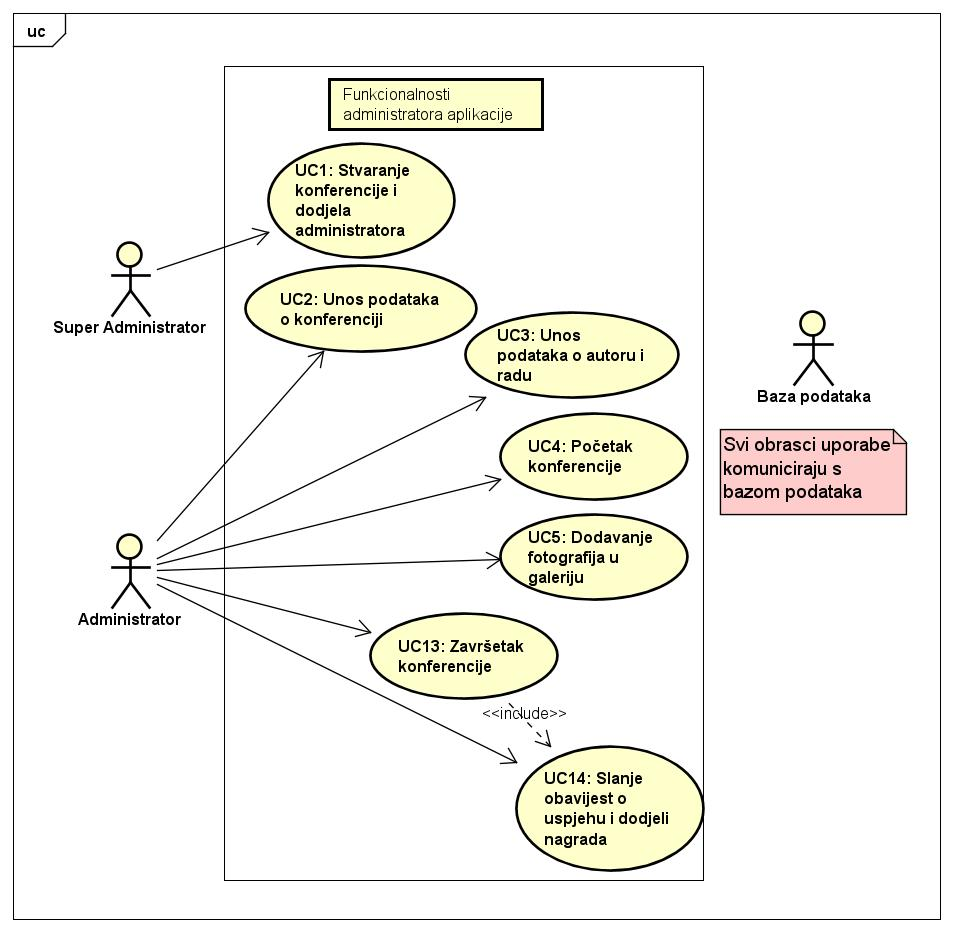
\includegraphics[scale=0.45]{dijagrami/UC_dijagram_administrator.JPG} %veličina slike u odnosu na originalnu datoteku i pozicija slike
						\centering
						\caption{Dijagram obrazaca uporabe - administrator}
						\label{fig:promjene}
					\end{figure}
					\begin{figure}[H]
						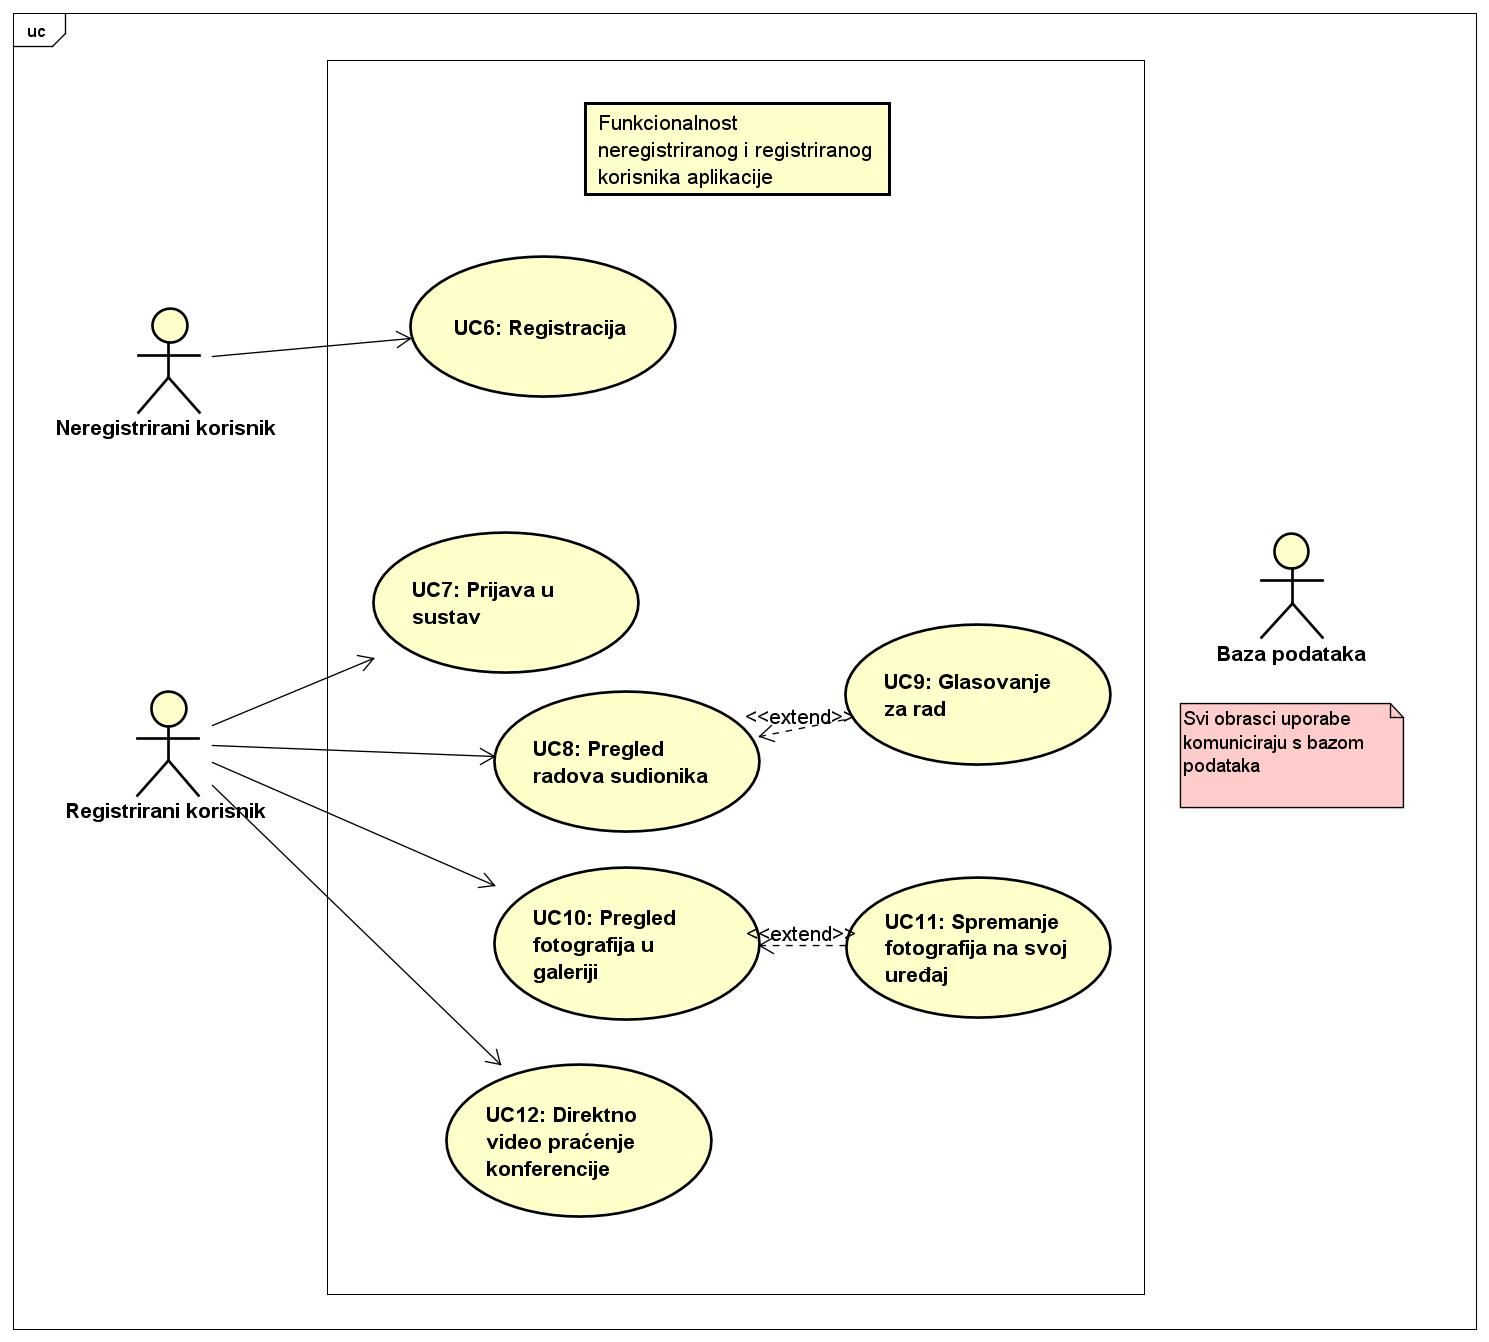
\includegraphics[scale=0.3]{dijagrami/UC_dijagram_korisnik.JPG} %veličina slike u odnosu na originalnu datoteku i pozicija slike
						\centering
						\caption{Dijagram obrazaca uporabe - korisnici}
						\label{fig:promjene2}
					\end{figure}
				\eject		
				
			\subsection{Sekvencijski dijagrami}
				\hspace{0.5cm} Korisnik pokreće aplikaciju. Ima ograničen pristup sadržajima aplikacije sve dok ne upiše pin koji je dodijeljen sudionicima konferencije. Upisani pin se zatim provjerava i korisnik nastavlja na stranicu za prijavu/registraciju.
				
				Kad korisnik ima stvoreni račun, prijavljuje se u aplikaciju pomoću adrese elektroničke pošte i lozinke. Prijavljeni korisnik onda može pristupiti sadržaju konferencije. 
				
				Za vrijeme sudjelovanja na konferenciji korisnik može pregledavati sadržaj konferencije i radove. Korisnik može glasovati samo za jedan rad i pratiti video prijenos trenutnih događanja u glavnoj konferencijskoj dvorani u realnom vremenu. Također ima dostupno pregledavanje i preuzimanje slika s konferencije - tijekom i nakon što konferencija završi. Korisnik može ugasiti aplikaciju kad god ima potrebu za tim. Zbog bolje preglednosti u dijagramu podrazumijevamo da radnje unutar konferencije korisnik može izvesti proizvoljnim redoslijedom dok na istoj sudjeluje.
				
				Dijagram je prikazan na sljedećoj stranici.
				\eject
				
				\begin{figure}[H]
					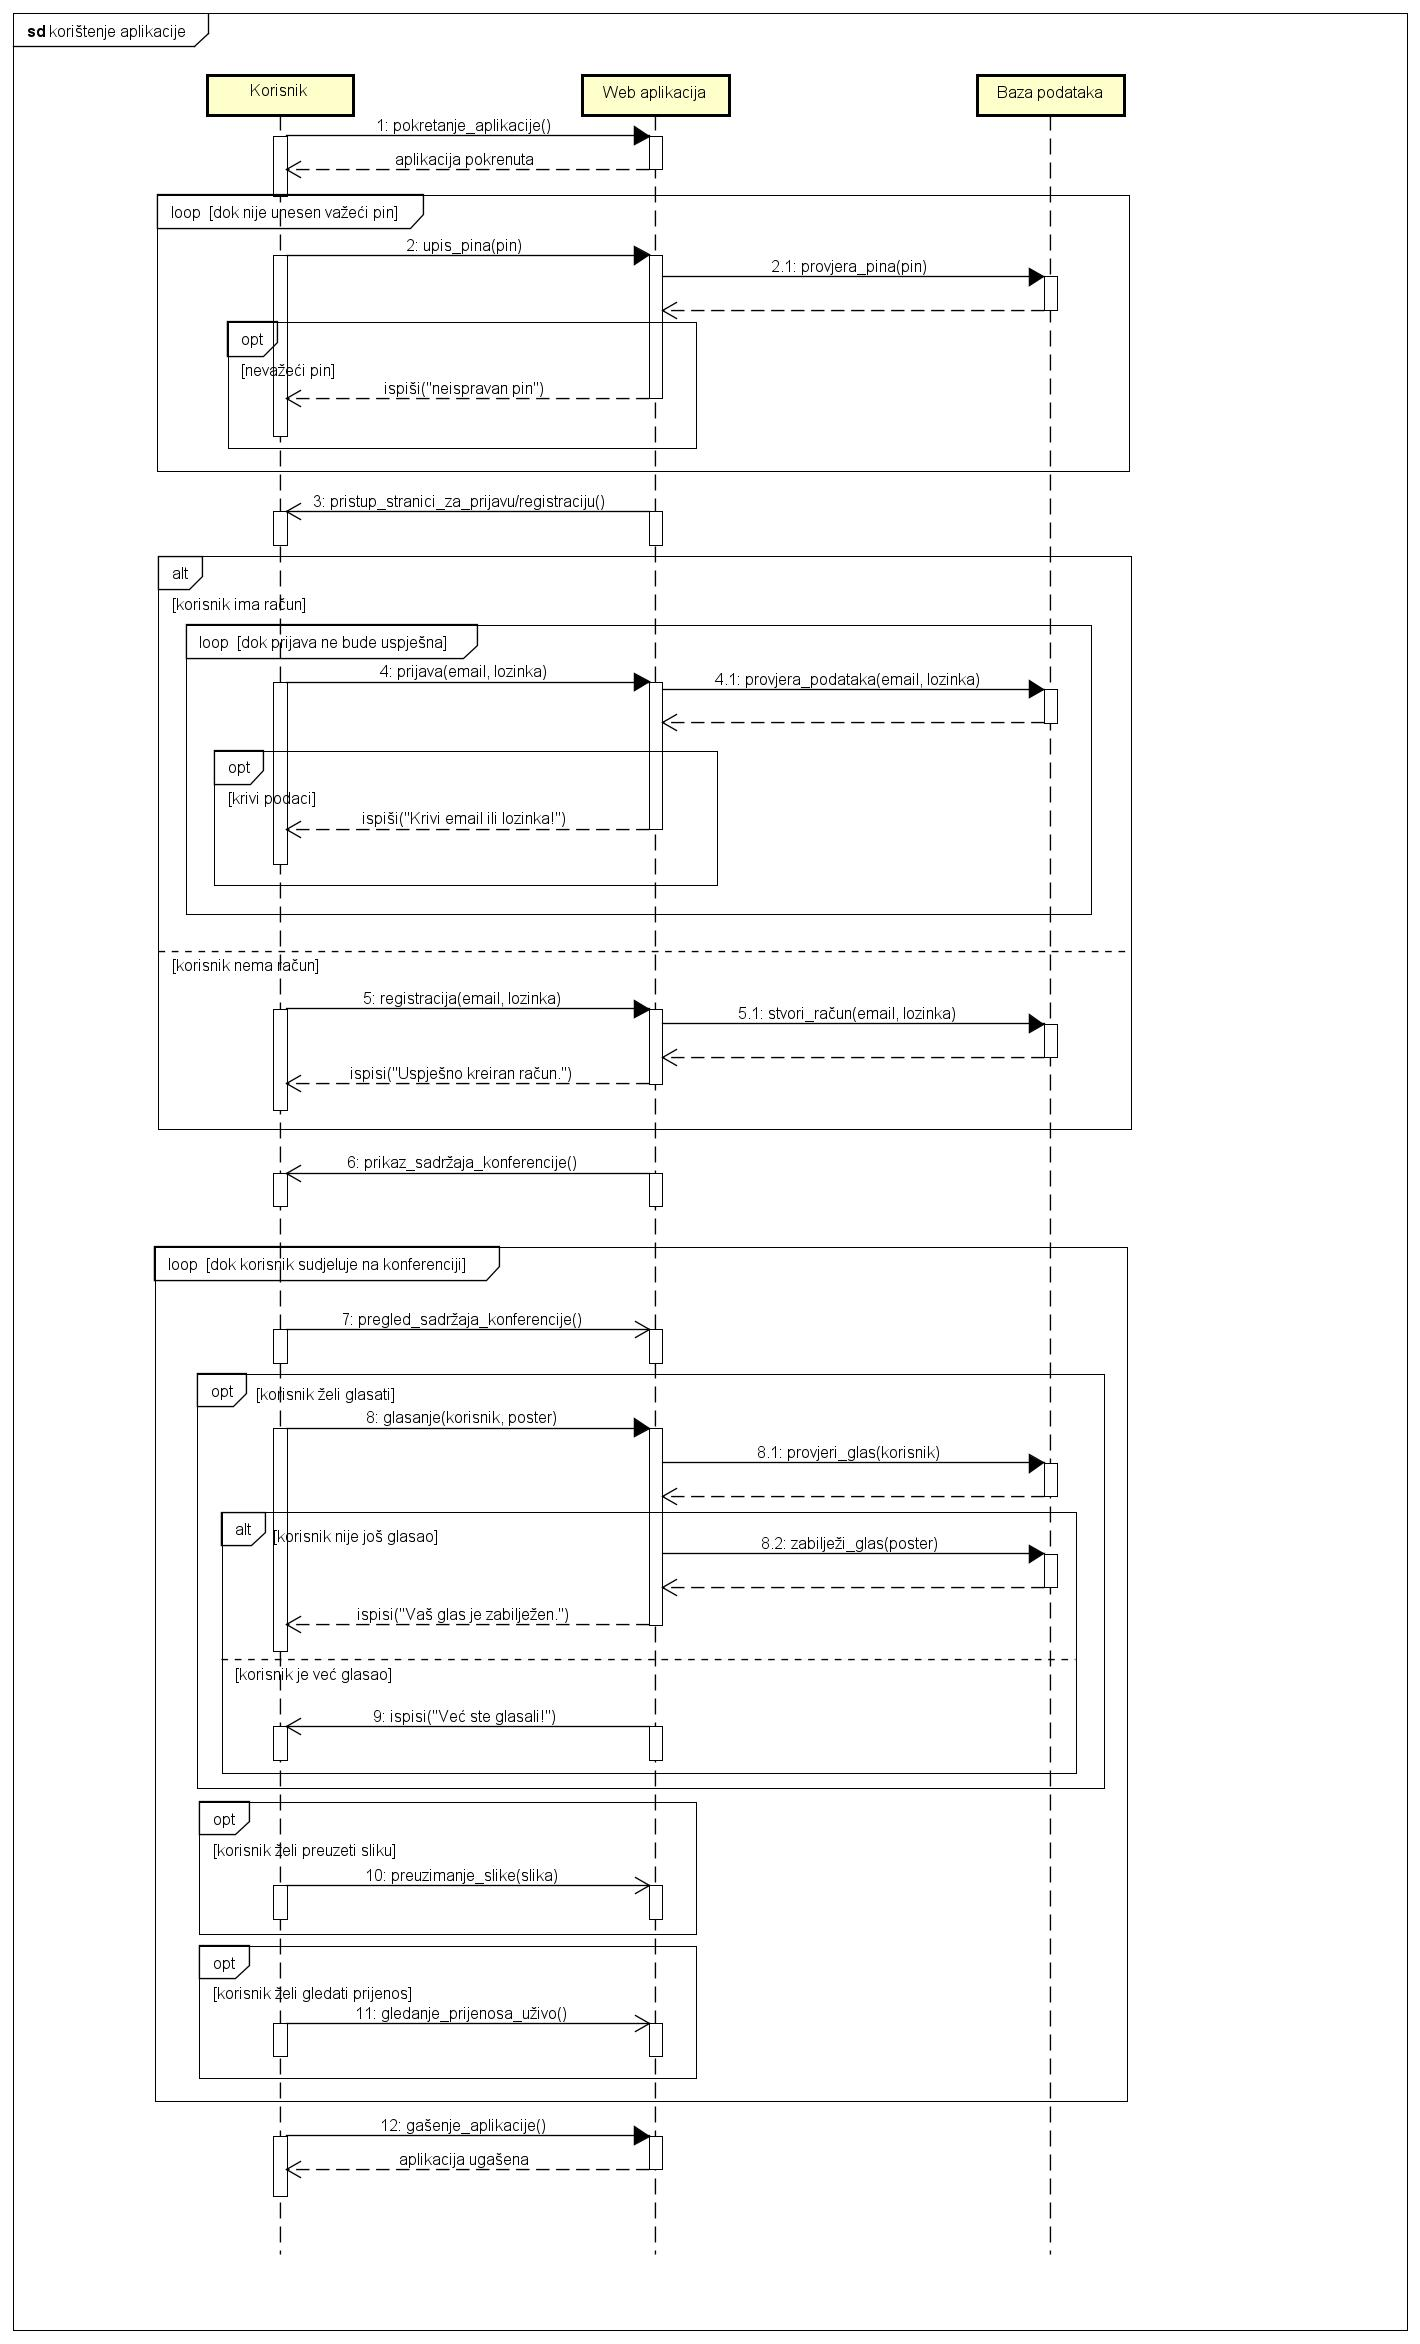
\includegraphics[scale=0.28]{dijagrami/koristenje_aplikacije.JPG} %veličina slike u odnosu na originalnu datoteku i pozicija slike
					\centering
					\caption{Sekvencijski dijagram korištenja aplikacije}
					\label{fig:promjene}
				\end{figure}

				Administrator dodaje autore i njihove radove prije početka konferencije. Nadodaje ih dok ne doda sve sudionike (autore) i njihove radove.
				Zatim dodaje sponzore konferencije dok ih sve ne upiše.

				Administrator započinje konferenciju. Tijekom konferencije administrator ima mogućnost dodavanja fotografija te konferencije. Administrator završava konferenciju. 

				Administrator dodaje fotografije i nakon konferencije.

				\begin{figure}[H]
					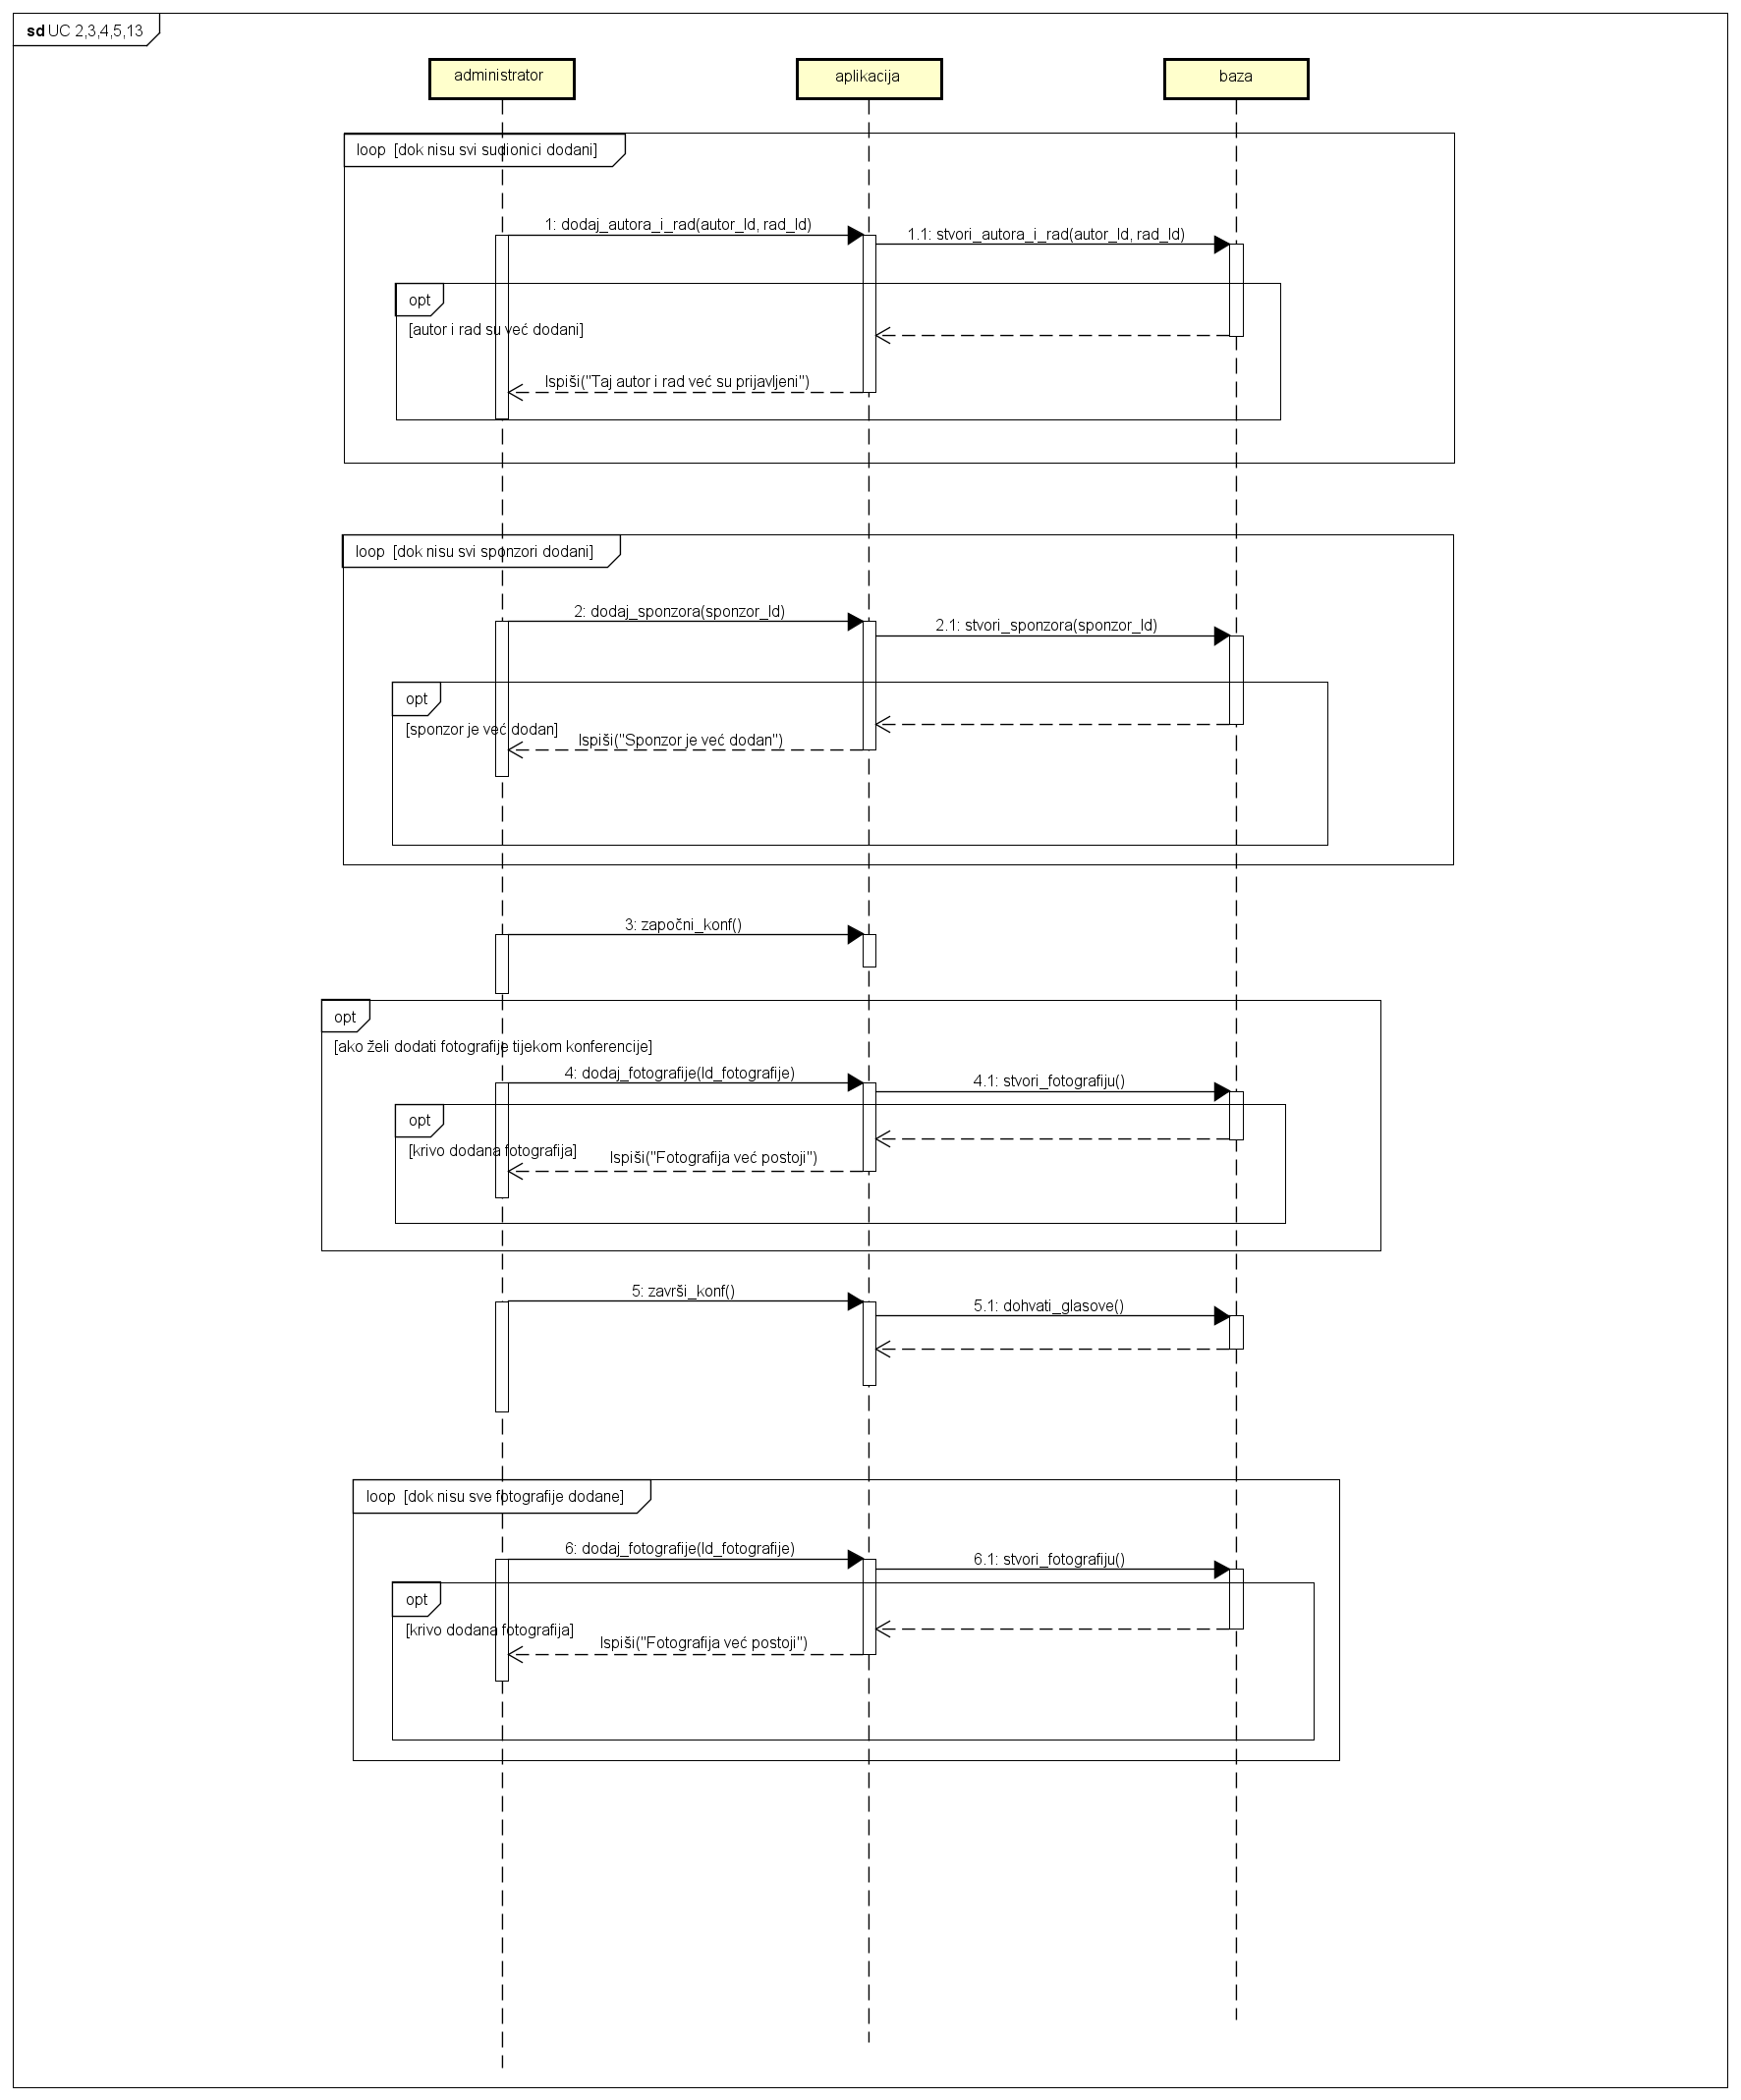
\includegraphics[scale=0.3]{dijagrami/sekv2.png}%veličina slike u odnosu na originalnu datoteku i pozicija slike
					\centering
					\caption{Sekvencijski dijagram korištenja aplikacije od strane administratora}
					\label{fig:promjene10}
				\end{figure}
				\eject
	
		\section{Ostali zahtjevi}
		
%			\textbf{\textit{dio 1. revizije}}\\
		 
			 \begin{packed_item}
				\item Sustav mora omogućiti istovremeni rad više korisnika u stvarnom vremenu
				\item Sustav i korisničko sučelje moraju podržavati znakovlje hrvatske abecede (dijakritičke znakove) prilikom prikazivanja tekstualnog sadržaja te unosa
				\item Pristupanje bazi podataka, tj. izvršavanje dijela programa u kojem se pristupa bazi podataka ne smije trajati duže od nekoliko sekundi
				\item Sustav treba biti implementiran kao web aplikacija koristeći objektno - orijentirane jezike
				\item Neispravnim korištenjem korisničkog sučelja, ne smije se narušiti funkcionalnost i rad sustava
				\item Sustav treba biti jednostavan i intuitivan za korištenje, odnosno korisnik ga mora moći koristiti bez korištenja (opširnih) uputa
				\item Prilikom nadogradnje sustava, ne smiju biti narušene njegove postojeće funkcionalnosti
				\item Veza s bazom podataka mora biti dobro zaštićena, brza i otporna na vanjske greške
				\item Sustav je responzivan na mobilnim uređajima
				\item Pristup sustavu treba biti omogućen iz javne mreže preko HTTPS protokola
			\end{packed_item}
			 
			 
			 
	